%%% XeLaTeX-article %%%
%# -*- coding: utf-8 -*-
%!TEX encoding = UTF-8 Unicode
%!TEX TS-program = xelatex  
%---------------------虽然加了%还是要保留!

\documentclass[17pt]{beamer}
\mode<presentation>
{
\usetheme[width=40pt]{Hannover}
\usecolortheme[]{dove}
\usefonttheme[]{structurebold}
\setbeameroption{hide notes}
}

\usepackage{fontspec}
\setmainfont{Arial} %设置主字体
\newfontfamily\sanskritfont[Script=Devanagari,Mapping=romantodevanagari,Scale=1.15]{Sanskrit 2003}             %输出天城体
%\newfontfamily\sanskritfont[Mapping=tex-text]{Times New Roman}              %输出转写
\doublehyphendemerits=-10000
\newcommand{\skt}[1]{{\sanskritfont{#1}}} %输出天城体
\newcommand{\skttrans}[1]{{\skt{#1}~#1}}  %输出天城体和转写
%----------------------------------------------------设置梵文输入方法 danda । ॥

\usepackage[UTF8,fontset=windows]{ctex}
\usepackage{amsmath}
%----------------------------------------------------设置中文环境

\usepackage{graphicx}
\usepackage{flafter} 
\graphicspath{{pic/}}
\usepackage{booktabs} 
\usepackage{nicematrix}
%-----------------------------------------插图表格

\usepackage{hyperref} 
\usepackage[dvipsnames]{xcolor}
\usepackage{colortbl}
\definecolor{light-gray}{gray}{0.9}
%------------------------------颜色

\newcommand{\verbroot}[1]{\textcolor{red}{$\sqrt{}$#1}}
\newcommand{\sktroot}[1]{{\verbroot{\skt{#1}}}}
\newcommand{\skttransroot}[1]{{\sktroot{#1}~\textcolor{red}{#1}}}
\newcommand{\nounstem}[1]{\textcolor{red}{#1\nobreakdash-}}
\newcommand{\sktnounstem}[1]{{\textcolor{red}{\skt{#1\nobreakdash-}}}}
\newcommand{\skttransnounstem}[1]{{\sktnounstem{#1}~\nounstem{#1}}}
\newcommand{\verbstem}[1]{\textcolor{blue}{#1\nobreakdash-}}
\newcommand{\sktverbstem}[1]{{\textcolor{blue}{\skt{#1\nobreakdash-}}}}
\newcommand{\skttransverbstem}[1]{{\sktverbstem{#1}~\verbstem{#1}}}
\newcommand{\wordending}[1]{\textcolor{Orange}{\nobreakdash-#1}}
\newcommand{\sktending}[1]{{\textcolor{Orange}{\skt{-#1}}}}
\newcommand{\skttransending}[1]{{\sktending{#1}~\wordending{#1}}}
\newcommand{\fullpada}[1]{\textcolor{OliveGreen}{#1}}
\newcommand{\sktpada}[1]{{\textcolor{OliveGreen}{\skt{#1}}}}
\newcommand{\skttranspada}[1]{{\sktpada{#1}~\fullpada{#1}}}

\newcommand{\veryimportant}[1]{\textcolor{red}{#1}}
\newcommand{\important}[1]{\textcolor{blue}{#1}}
\newcommand{\notsoimportant}[1]{\textcolor{gray}{#1}}
%-------------------------------------------词根等标颜色

\title{{梵语提高}}
\subtitle{18. 不带插入元音的动词语干}
\author[张雪杉]{文学院~~张雪杉 \\ zhangxueshan@sdnu.edu.cn}
\date{}
%\institute{}


\begin{document}


\begin{frame}
  \titlepage
\end{frame}

\begin{frame}
  \frametitle{本节内容}
  \tableofcontents
\end{frame}

\section{动词复习}
\begin{frame}{复习~~带插入元音的语干}
  \small
  \raggedright
  词干都是以\nobreakdash-a\nobreakdash-结尾
  \begin{itemize}
    \item 第一类:元音二合后加\nobreakdash-a\nobreakdash-
    \verbroot{bhṛ}  \verbstem{bhara}
    \item 第四类:加\nobreakdash-ya\nobreakdash-
    \verbroot{hṛṣ}  \verbstem{hṛṣya}
    \item 第六类:加\nobreakdash-a\nobreakdash-
    \verbroot{likh}  \verbstem{likha}
    \item 第十类:加\nobreakdash-aya\nobreakdash-
    \verbroot{cur}  \verbstem{coraya}
    \end{itemize}
\end{frame}

\begin{frame}{现在时语尾}
  \centering
  \begin{tabular}{@{}llll@{}} % 4 columns
    & 单数  & 双数  & 复数 \\
    第一人称 & \wordending{mi} & \wordending{vaḥ}  & \wordending{maḥ}  \\
    第二人称 & \wordending{si} & \wordending{thaḥ} & \wordending{tha}  \\
    第三人称 & \wordending{ti} & \wordending{taḥ} & \wordending{\important{a}nti}  \\
  \end{tabular}   
\end{frame}

\section{不带插入元音的动词语干}
\begin{frame}{\insertsection }
    \tableofcontents[currentsection]
\end{frame}

\subsection{语干组成}
\begin{frame}{\insertsubsection }
  \begin{itemize}
    \item 不带插入元音的语干有强弱之分
    \item 强语干二合,弱语干零级
  \end{itemize}
\end{frame}

\begin{frame}{例词大表}
    \centering    
    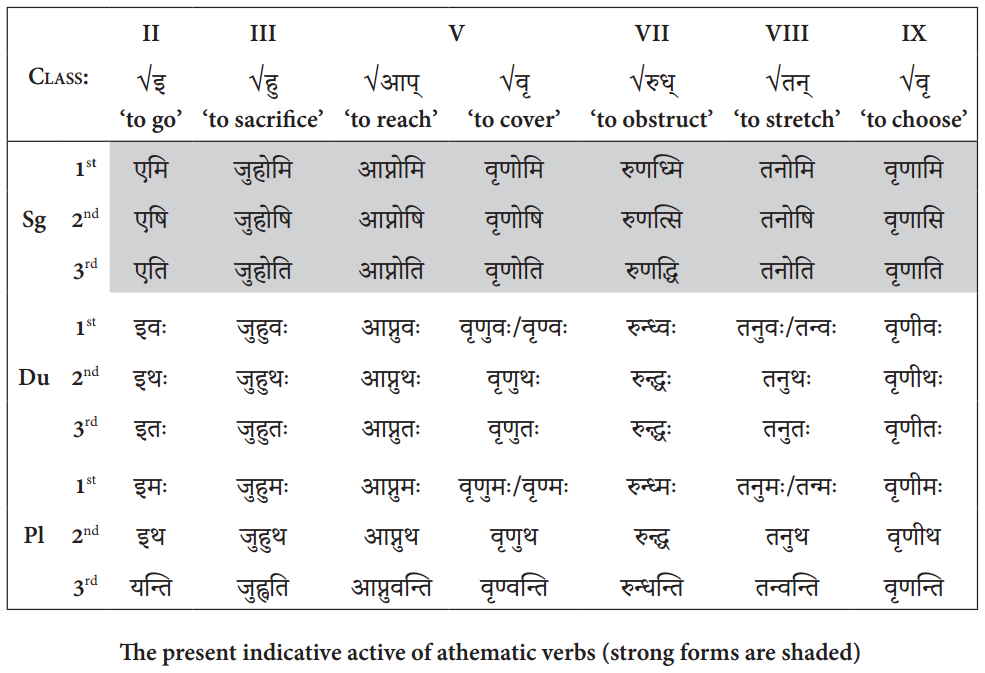
\includegraphics[width=\textwidth]{athematicverb.png}
\end{frame}

\subsection{第二类动词}
\begin{frame}%[fragile]
  \frametitle{\insertsubsection ~~ \verbroot{i} 走}
  \begin{itemize}
    \item 词根直接加词尾
  \end{itemize}
  \centering
  \begin{NiceTabular}{llll}
    \CodeBefore
      \rectanglecolor{light-gray}{2-2}{4-2}
    \Body % 7 columns
    & 单  & 双 & 复  \\
    1 & \fullpada{emi} & \fullpada{ivaḥ} & \fullpada{imaḥ} \\
    2 & \fullpada{eṣi}  & \fullpada{ithaḥ} & \fullpada{itha} \\
    3 & \fullpada{eti} & \fullpada{itaḥ} & \fullpada{\important{y}anti}  \\
  \end{NiceTabular}   
\end{frame}

\subsection{第三类动词}
\begin{frame}%[fragile]
  \frametitle{\insertsubsection ~~ \verbroot{hu} 祭}
  \begin{itemize}
    \item 重复语干加词尾
    \item 第三人称复数词尾用\wordending{ati}
  \end{itemize}
  \centering
  \begin{NiceTabular}{llll}
    \CodeBefore
      \rectanglecolor{light-gray}{2-2}{4-2}
    \Body % 7 columns
    & 单  & 双 & 复  \\
    1 & \fullpada{juhomi} & \fullpada{juhuvaḥ} & \fullpada{juhumaḥ} \\
    2 & \fullpada{juhoṣi}  & \fullpada{juhuthaḥ} & \fullpada{juhutha} \\
    3 & \fullpada{juhoti} & \fullpada{juhutaḥ} & \fullpada{juh\important{v}\textcolor{Orange}{ati}}  \\
  \end{NiceTabular}   
\end{frame}

\begin{frame}[fragile]{\insertsubsection ~~重复规则}
  \small
  \begin{itemize}
    \item 重复音节=第一个辅音+第一个元音 
    \verbroot{takṣ} \verbstem{ta\nobreakdash-takṣ} ~~\verbroot{kram} \verbstem{ca-kram}
    \item 元音特殊规则
    \begin{itemize}
      \item 长元音变短 \verbroot{dā} \verbstem{da-dā}
    \end{itemize}
    \item 辅音特殊规则
    \begin{itemize}  
      \item 送气变不送气 \verbroot{dhā} \verbstem{da-dhā}
      \item 喉音变腭音 \verbroot{gup} \verbstem{ju-gup}
      \item h(*gh)变j \verbroot{hu} \verbstem{ju-hu}
      \item 复合咝音不重复 \verbroot{stubh} \verbstem{tu-stubh}
    \end{itemize}
  \end{itemize}
\end{frame}

\subsection{第五类动词}
\begin{frame}%[fragile]
  \frametitle{\insertsubsection }
  \small
  \begin{itemize}
    \item 词根不变,强语干加\nobreakdash-no\nobreakdash-,弱语干加\nobreakdash-nu\nobreakdash-
  \end{itemize}
  \centering
  \begin{NiceTabular}{llll}
    \CodeBefore
      \rectanglecolor{light-gray}{2-2}{4-2}
    \Body % 7 columns
    &   \multicolumn{3}{c}{\verbroot{āp}}  \\
    1 & \fullpada{āpnomi} & \fullpada{āpnuvaḥ} & \fullpada{āpnumaḥ} \\
    2 & \fullpada{āpnoṣi}  & \fullpada{āpnuthaḥ} & \fullpada{āpnutha} \\
    3 & \fullpada{āpnoti} & \fullpada{āpnutaḥ} & \fullpada{āpn\important{uv}anti}  \\
  \end{NiceTabular} 
  \begin{itemize}
    \item 第一人称双数复数的u可能省略
  \end{itemize}
  \begin{NiceTabular}{llcc}
    \CodeBefore
      \rectanglecolor{light-gray}{2-2}{4-2}
    \Body % 7 columns
    &    \multicolumn{3}{c}{\verbroot{vṛ}} \\
    1  & \fullpada{vṛṇomi} & \fullpada{vṛṇuvaḥ/vṛṇvaḥ} & \fullpada{vṛṇumaḥ/vṛṇmaḥ} \\
    2 & \fullpada{vṛṇoṣi}  & \fullpada{vṛṇuthaḥ} & \fullpada{vṛṇutha} \\
    3  & \fullpada{vṛṇoti} & \fullpada{vṛṇotaḥ} & \fullpada{vṛṇ\important{v}anti}  \\
  \end{NiceTabular}   
\end{frame}

\subsection{第七类动词}
\begin{frame}%[fragile]
  \frametitle{\insertsubsection ~~ \verbroot{rudh} 阻}
  \begin{itemize}
    \item 强加\nobreakdash-na\nobreakdash-弱加\nobreakdash-n\nobreakdash-,加在落尾辅音前
  \end{itemize}
  \centering
  \begin{NiceTabular}{llll}
    \CodeBefore
      \rectanglecolor{light-gray}{2-2}{4-2}
    \Body % 7 columns
    & 单  & 双 & 复  \\
    1 & \fullpada{ruṇadhmi} & \fullpada{rundhvaḥ} & \fullpada{rundhmaḥ} \\
    2 & \fullpada{ruṇatsi}  & \fullpada{runddhaḥ} & \fullpada{runddha} \\
    3 & \fullpada{ruṇaddhi} & \fullpada{runddhaḥ} & \fullpada{rundhanti}  \\
  \end{NiceTabular}   
\end{frame}

\begin{frame}{相关连声}
  \small
  \begin{itemize}
    \item n随后音换行
    
    \verbroot{yuj(VII)} 1st. Du. \fullpada{yuñjvaḥ}
    \item s前浊音和送气都失去 
    
    \verbroot{rudh(VII)} 2nd. Sg. \fullpada{ruṇatsi}
    \item 爆破音前浊音或送气失去 
    
    \verbroot{chid(VII)} 3rd. Sg. \fullpada{chinatti}
    \item buddha连声 
    
    \verbroot{rudh(VII)} 3rd. Sg. \fullpada{ruṇaddhi}
    \item 腭音变喉音 \verbroot{vac(II)} 3rd. Sg. \fullpada{vakti}
    
  \end{itemize}
\end{frame}

\subsection{第八类动词}
\begin{frame}%[fragile]
  \frametitle{\insertsubsection ~~ \verbroot{tan} 阻}
  \small
  \begin{itemize}
    \item 强语干加\nobreakdash-o\nobreakdash-弱语干加\nobreakdash-u\nobreakdash-
    \item 大部分词根以\nobreakdash-n结尾,所以和第五类很像
  \end{itemize}
  \centering
  \begin{NiceTabular}{llcc}
    \CodeBefore
      \rectanglecolor{light-gray}{2-2}{4-2}
    \Body % 7 columns
    & 单  & 双 & 复  \\
    1 & \fullpada{tanomi} & \fullpada{tanuvaḥ/tanvaḥ} & \fullpada{tanumaḥ/tanmas} \\
    2 & \fullpada{tanoṣi}  & \fullpada{tanuthaḥ} & \fullpada{tanutha} \\
    3 & \fullpada{tanoti} & \fullpada{tanutaḥ} & \fullpada{tanvanti}  \\
  \end{NiceTabular}   
\end{frame}

\subsection{第九类动词}
\begin{frame}%[fragile]
  \frametitle{\insertsubsection ~~ \verbroot{vṛ} 选}
  \begin{itemize}
    \item 强语干加\nobreakdash-nā\nobreakdash-,弱语干加\nobreakdash-nī\nobreakdash-/\nobreakdash-n\nobreakdash-
  \end{itemize}
  \centering
  \begin{NiceTabular}{llll}
    \CodeBefore
      \rectanglecolor{light-gray}{2-2}{4-2}
    \Body % 7 columns
    & 单  & 双 & 复  \\
    1 & \fullpada{vṛṇāmi} & \fullpada{vṛṇīvaḥ} & \fullpada{vṛṇīmaḥ} \\
    2 & \fullpada{vṛṇāsi}  & \fullpada{vṛṇīthaḥ} & \fullpada{vṛṇītha} \\
    3 & \fullpada{vṛṇāti} & \fullpada{vṛṇītaḥ} & \fullpada{vṛṇanti}  \\
  \end{NiceTabular}   
\end{frame}

\subsection{总结}
\begin{frame}{总结}
  \small
  \raggedright
  \begin{itemize}
    \item 第二类:词根直接加词尾
    \item 第三类:重复语干加词尾
    \item 第五类:强语干加\nobreakdash-no\nobreakdash-,弱语干加\nobreakdash-nu\nobreakdash-
    \item 第七类:强加\nobreakdash-na\nobreakdash-弱加\nobreakdash-n\nobreakdash-,
    
    \hspace*{4em}加在落尾辅音前
    \item 第八类:强语干加\nobreakdash-o\nobreakdash-,弱语干加\nobreakdash-u\nobreakdash-
    \item 第九类:强语干加\nobreakdash-nā\nobreakdash-,弱语干加\nobreakdash-nī\nobreakdash-/\nobreakdash-n\nobreakdash-
  \end{itemize}
\end{frame}

\section{本节作业}

\begin{frame}{\insertsection }
  \begin{itemize}
    \item
      第十八章练习3
    \item
      勘误:第2题\skt{vesīti}改为\skt{vetsīti}
    \bigskip
    %\item
    %  现在请做学习通\nobreakdash-章节\nobreakdash-课后问卷
  \end{itemize}
\end{frame}  

\end{document}	
